\documentclass[handout]{beamer}

\usepackage{Vor2018glærur}

\title{Tölvunarfræði 2}
\subtitle{Vika 1}

\begin{document}

\begin{frame}
\titlepage
\end{frame}

\section{Um námskeiðið}

\begin{frame}{Allar upplýsingar}
Allar tiltækar upplýsingar um námskeiðið má finna í Syllabus.pdf. Skjalið er á Piazza, undir resources.
\end{frame}

\section{C++ og þýðing}

\begin{frame}{C++}
    \begin{itemize}
        \item C++ er almennt forritunarmál, notað á ýmsum sviðum
        \item Yfirleitt litið á það sem ``mid-level'' forritunarmál í dag
    \begin{itemize}
        \item Höfum ýmis þægindi sem við búumst við af nútímaforritunarmálum
        \item Höfum líka ýmsa möguleika á beinni minnisstjórnun
    \end{itemize}
        \item Kom út snemma á 9. áratugnum
    \end{itemize}
\end{frame}

\begin{frame}{Af hverju C++?}
    \begin{itemize}
        \item Mörg mikilvæg tölvunarfræðihugtök sem eru vel sýnileg í C++
        \item Málið hefur verið mjög áhrifamikið í málum sem á eftir koma
        \item Praktískt, líklegt að fólk sem vinnur við forritun muni rekast á C-mál
    \end{itemize}
\end{frame}


\begin{frame}[fragile]{Hello World forrit í C++}
    Hið hefðbundna forrit sem skrifar út ``halló heimur'', í C++:
    \cppfile[label=hello.cpp]{Code/w1/hello.cpp}
    Þessa skrá mætti búa til í hvaða textaritli (e. \emph{plaintext editor}) sem er.
\end{frame}

\begin{frame}[fragile]{Hvað erum við að horfa á?}
    \begin{itemize}
        \item \texttt{\#include <iostream>}: Veitir okkur aðgang að staðalstraumum
        \item \texttt{int main()}: Skilgreining falls að nafni \texttt{main} sem tekur engin inntök og skilar heiltölu
        \begin{itemize}
            \item Afmarkað með slaufusvigum
        \end{itemize}
        \item \verb|std::cout << "Halló heimur!" << std::endl;|: Strengurinn ``halló heimur'' skrifaður á ``console out'' strauminn með straumsinnsetningarvirkjanum \verb|<<| ásamt boðum um að línunni sé lokið
    \end{itemize}
\end{frame}

\begin{frame}[fragile]{Þýðing C++ forrits}
    C++ kóði er undantekningalítið þýddur. Dæmi um þýðanda er \href{https://gcc.gnu.org/}{GCC}, sem kalla má á af skipanalínu:
    \begin{minted}[frame=lines]{bash}
$ g++ hello.cpp -o hello
$ ./hello
Halló heimur!
    \end{minted}
    Hér er \texttt{g++} skipunin sem keyrir upp GCC þýðandann fyrir forritskóðaskrána \texttt{hello.cpp} og býr til keyranlegu skrána \texttt{hello}.
\end{frame}

\begin{frame}[fragile]{Hvar er þessi þýðandi keyrður?}
    \begin{itemize}
        \item Sýnidæmi gera ráð fyrir notkun á skipanalínu \eng{command line}
        \begin{itemize}
            \item Á Windows: keyra cmd.exe
            \item Á Mökkum: finna terminal
            \item Á Linux: Ýmis nöfn, en á að vera auðfinnanlegt
        \end{itemize}
        \item Hægt er að athuga hvort að GCC sé uppsett með því að keyra
    \end{itemize}
    \begin{minted}[frame=lines]{bash}
$ g++ --version
g++ (Ubuntu 6.3.0-12ubuntu2) 6.3.0 20170406
    \end{minted}
\end{frame}

\begin{frame}{Undir húddinu}
\begin{columns}
\column{0.66\textwidth}
    Það að mynda keyrsluskrá út frá C++ kóða fer fram í nokkrum (hér einfölduðum) skrefum.
    \begin{enumerate}
        \item Forritskóðinn fer í gegnum forþýðanda (e. \emph{preprocessor}), sem sækir \texttt{\#include}-aðan kóða, framkvæmir textaútskiptingar o.fl.
        \item Útvíkkaði kóðinn er þýddur (e. \emph{compiled})
        \item Þýddi kóðinn er tengdur (e. \emph{linked}) svo úr verði keyranleg skrá
    \end{enumerate}
\column{0.33\textwidth}
\begin{center}
    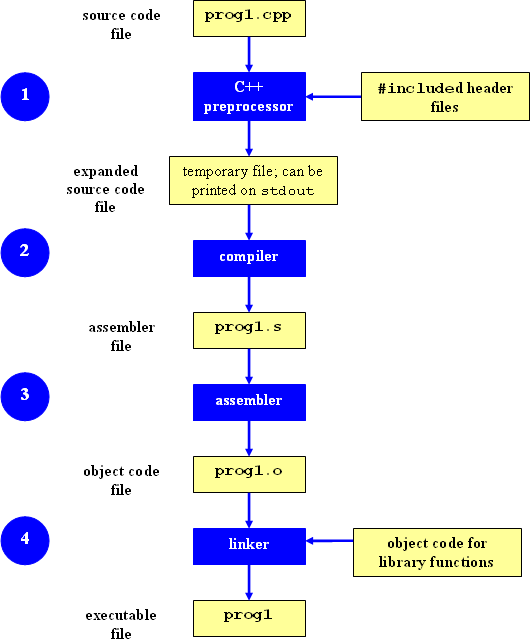
\includegraphics[width=1.1\linewidth]{compile}\\
    {\tiny \href{http://faculty.cs.niu.edu/~mcmahon/CS241/Notes/compile.html}{Útskýring/uppruni myndar} }
\end{center}
\end{columns}
\end{frame}

\begin{frame}[fragile]{Að skoða milliskrár}
Við getum stöðvað GCC á ýmsum stigum.

Stöðvað eftir forþýðingu, skrifar oft út mikinn textavegg:
\begin{minted}[frame=lines]{bash}
$ g++ -E p.cpp
\end{minted}
Fá smalamálsframsetningu sem þýðandinn býr til í skrána \texttt{p.s}:
\begin{minted}[frame=lines]{bash}
$ g++ -S p.cpp
\end{minted}
Sleppa tengingu, fá ``object code'' í skrána \texttt{p.o}:
\begin{minted}[frame=lines]{bash}
$ g++ -c p.cpp
\end{minted}
\end{frame}

\begin{frame}{Uppsetning GCC}
    Vísi að uppsetningarleiðbeiningum má finna á verkefnislýsingu skilaverkefnis 0. Dæmatímakennarar geta aðstoðað við uppsetningu \emph{en reynið til hins ýtrasta að setja þýðandann upp sjálf.}
    \begin{center}
        \begin{tabular}{llll}
            \toprule
            Hópur&Tími&Kennari&Stýrikerfi\\
            \midrule
            d1&Mán 15:00&Kristján&Windows\\
            d3&Mán 16:40&Jón&OS X\\
            d4&Þri 15:00&Einar&OS X\\
            d5&Þri 15:50&Freyr&OS X\\
            d6&Mán 15:00&Sigurður&Windows\\
            \bottomrule
        \end{tabular}
    \end{center}
\end{frame}

\begin{frame}{Ritlar og þróunarumhverfi}
    Val á ritli og/eða þróunarumhverfi fyrir C++ skiptir ekki höfuðmáli í þessu námskeiði. Vitað er að \href{https://code.visualstudio.com/}{Microsoft VS Code} `virkar''.

    \begin{center}
        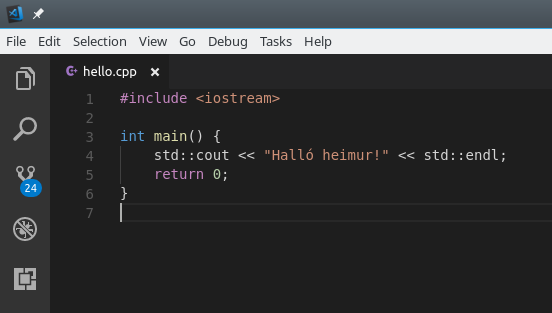
\includegraphics[width=0.6\linewidth]{vscode-hello-world}
    \end{center}
\end{frame}

\section{Málfræði C++}

\begin{frame}[fragile]{Grundvallarmálfræði}
Mikið af grundvallarmálfræði (en ekki allri virkni!) C++ ætti að vera kunnuglegt þeim sem þekkja til Java.
\begin{columns}
    \column{0.6\textwidth}
    \cppfile[firstline=5,lastline=10,gobble=4,fontsize=\small, linenos=false]{Code/w1/javacomparison.cpp}
    \column{0.4\textwidth}
    \cppfile[firstline=13,lastline=15,fontsize=\small, linenos=false]{Code/w1/javacomparison.cpp}
\end{columns}
Leggjum héðan af áherslu á þá hluta sem eru öðru vísi en í Java.
\end{frame}

\begin{frame}{\#include}
\begin{itemize}
    \item Í C++ hefjast skipanir til forþýðandans á \#
    \item Það sem við gerum langoftast er:
    \begin{itemize}
        \item ``Taktu skipanir úr þessari skrá og settu þær hingað''
        \item Höfum þegar séð skipunina \texttt{\#include <iostream>}
    \end{itemize}
    \item \texttt{\#include} vinnur á hausskrám (e. \emph{header files}), sem innihalda forritslýsingar
    \item Útfærslan á þeim forritum sem er síðan ``annars staðar'' og er tengdar seinna
\end{itemize}
\end{frame}

\begin{frame}{Nafnarými}
    \texttt{cout} skipunin (og mun fleiri) eru í \texttt{std} nafnarýminu (e. \emph{namespace}). Við getum sagt þýðandanum að leita í ákveðnum nafnarýmum:
    \cppfile[label=namespace.cpp]{Code/w1/namespace.cpp}
\end{frame}

\begin{frame}{Nákvæmari innflutningur}
\cppfile[label=namespacespecific.cpp]{Code/w1/namespacespecific.cpp}
\end{frame}

\section{Straumar, inntak og úttak}

\begin{frame}{Inntak og úttak}
    Í C++ eru straumarnir mjög sýnilegir.
    \cppfile[label=input.cpp, firstline=7, lastline=16, gobble=4, fontsize=\small]{Code/w1/input.cpp}
\end{frame}

\begin{frame}[fragile]{Skipanalínan}
Skipanalína og straumar virka vel saman.
\begin{columns}
    \column{0.3\textwidth}
    \inputminted[frame=lines,label=numbers.txt]{bash}{Code/w1/numbers.txt}
    \column{0.6\textwidth}
    \cppfile[firstline=6, lastline=11, gobble=4, label=loopyinput.cpp]{Code/w1/loopyinput.cpp}
\end{columns}
\begin{minted}[frame=lines]{bash}
$ ./loopyinput < numbers.txt
29
\end{minted}
\end{frame}

\begin{frame}[fragile]{Skilatáknið}
    \begin{itemize}
        \item Hvað þýðir þetta \texttt{return 0;} neðst í \texttt{main}-föllunum? \pause
        \begin{itemize}
            \item Talan sem \texttt{main} skilar er skilatákn \eng{exit code} forritsins
        \end{itemize}
        \item Skil á tölunni 0 tákna að fallið hafi lokið keyrslu rétt, hærri tölur tákna einhvers konar vandræði
            \begin{itemize}
                \item Sjá: \texttt{/usr/include/sysexits.h}
            \end{itemize}
        \item Önnur forrit geta notað skilatáknið til að ákveða keyrslu
        \item Í bash er síðasta skilatákn aðgengilegt með \texttt{\$?}, í cmd.exe með \texttt{ERRORLEVEL}
    \end{itemize}
\begin{minted}[frame=lines]{bash}
$ g++ hello.cpp -o hello
$ echo $?
0
\end{minted}
\end{frame}

\section{Inngangur að fylkjum og strengjum}

\begin{frame}[fragile]{Fylki}
    Líkt og í Java eru venjuleg fylki af fastri stærð. Þýðandinn tekur frá minnisblokk af ákveðinni stærð fyrir fylki og notar fjarlægðina frá upphafi blokkarinnar til að vísa í stök fylkisins.

    Dæmi um fylki:
    \begin{minted}[frame=lines]{cpp}
int numbers1[5] = {}; // initializes all integers to 0
int numbers2[5] = {34, 56, -21, 5002, 365};
int numbers3[] = {2016, 2052, -525}; // 3 elements
    \end{minted}
    Vísar í fylki í C++ byrja í 0.

\end{frame}

\begin{frame}{Varúð!}
    C++ forrit þýðast og keyrast þó vísað sé út fyrir fylki.
    \cppfile[firstline=3, label=arraydanger.cpp]{Code/w1/arraydanger.cpp}
\end{frame}

\begin{frame}{Strengir}
    C++ getur unnið með strengi eins og þeir eru í forritunarmálinu C - fylki af táknum. Strengirnir sem við höfum séð hingað til hafa flestir verið af slíkri gerð.
    \cppfile[firstline=6, lastline=12, fontsize=\small, gobble=4, label=nullterm.cpp]{Code/w1/nullterm.cpp}
    Strengjunum er ``lokað'' með sértákninu \texttt{'\textbackslash0'}. Strengjavinnsla hættir á þeim stað.
\end{frame}

\section{Inngangur að bendum}

\begin{frame}{Bendar}
\begin{itemize}
 \item Bendir er breyta sem inniheldur staðsetningu minnissvæðis
 \begin{itemize}
  \item Hún ``bendir á'' minnissvæðið
 \end{itemize}
 \item Hægt er að nota bendinn til að fá aðgang að gögnunum sem geymd eru í minnissvæðinu
\end{itemize}
\begin{center}
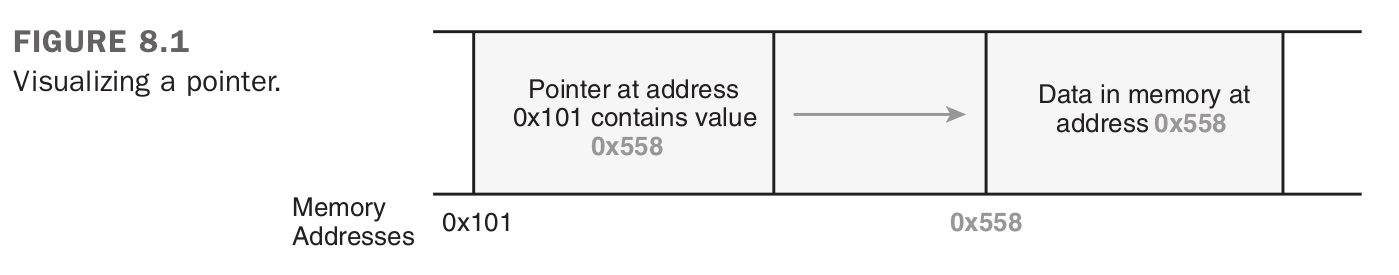
\includegraphics[width=\textwidth]{pointer-visualization}
\end{center}
\end{frame}

\begin{frame}[fragile]{Bendar}
    Hægt er að ná í staðsetningu minnissvæðis með \texttt{\&} virkjanum. Notum stjörnu (\texttt{*}) á milli skilgreiningar á taginu og breytuheitisins til að skilgreina bendi.
    \cppfile[firstline=6, lastline=10, gobble=4, fontsize=\small, label=pointerintro.cpp]{Code/w1/pointerintro.cpp}
    Oftast fáum við benda þegar við úthlutum minni sérstaklega. 
    
    Sjá síðar: \texttt{new}.
\end{frame}

\begin{frame}[fragile]{Bendar}
    Við getum sótt gögn sem bendir vísar á með \texttt{*} virkjanum.
    \cppfile[firstline=6, lastline=15, gobble=4, fontsize=\small, label=dereferencing.cpp]{Code/w1/dereferencing.cpp}
\end{frame}


\section{Lokaorð}

\begin{frame}{Þessi glærupakki}
    Öll nafngreind forrit í þessum glærupakka, ásamt glærupakkanum sjálfum, má finna á  \href{https://github.com/Ernir/kennsluefni/tree/master/T2/Code/w1}{Github}.
\end{frame}


\begin{frame}{Næst}
    Meira um minnismódelið í C++, hlutbundin forritun í C++.
\end{frame}


\end{document}
